\documentclass[11pt,twocolumn,a4paper]{article}

\usepackage[utf8]{inputenc}
\usepackage[T1]{fontenc}
\usepackage{amsmath,amssymb,amsthm,mathtools}
\usepackage{bm}
\usepackage{physics}
\usepackage{graphicx}
\usepackage{hyperref}
\usepackage{cleveref}
\usepackage[margin=2.2cm]{geometry}
\usepackage{enumitem}
\usepackage{float}
\usepackage{booktabs}
\usepackage{natbib}
\usepackage{algorithm}
\usepackage{algorithmic}
\usepackage{listings}
\usepackage{xcolor}
\usepackage{caption}
\usepackage{microtype}
\usepackage{lmodern}
\usepackage{tikz}
\usetikzlibrary{arrows.meta,positioning,shapes.geometric,fit,calc}

\newtheorem{theorem}{Theorem}[section]
\newtheorem{lemma}[theorem]{Lemma}
\newtheorem{corollary}[theorem]{Corollary}
\newtheorem{proposition}[theorem]{Proposition}
\theoremstyle{definition}
\newtheorem{definition}[theorem]{Definition}
\newtheorem{axiom}{Axiom}
\newtheorem{construction}[theorem]{Construction}
\theoremstyle{remark}
\newtheorem{remark}[theorem]{Remark}
\newtheorem{example}[theorem]{Example}

\newcommand{\kB}{k_{\mathrm{B}}}
\newcommand{\Sk}{S_{\mathrm{k}}}
\newcommand{\St}{S_{\mathrm{t}}}
\newcommand{\Se}{S_{\mathrm{e}}}
\newcommand{\Sspace}{\mathcal{S}}
\newcommand{\Scoord}{\mathbf{S}}
\newcommand{\R}{\mathbb{R}}
\newcommand{\Z}{\mathbb{Z}}
\newcommand{\N}{\mathbb{N}}
\newcommand{\Recv}{\mathcal{R}}
\newcommand{\Floor}{\mathfrak{S}_{\mathrm{floor}}}
\newcommand{\Osc}{\mathfrak{O}}
\newcommand{\Cat}{\mathfrak{C}}
\newcommand{\Part}{\mathfrak{P}}
\newcommand{\Reps}{\mathfrak{R}}
\newcommand{\eval}{\mathrm{eval}}
\newcommand{\Sexp}{\xi}
\newcommand{\Sig}{\Sigma}
\newcommand{\Tree}{\mathcal{T}}
\newcommand{\Leaf}{\mathcal{L}}
\newcommand{\trit}{\mathsf{t}}
\newcommand{\addr}{\mathbf{a}}
\newcommand{\dcat}{d_{\mathrm{cat}}}
\newcommand{\orderpar}{r}
\newcommand{\coupmat}{\mathbf{K}}
\newcommand{\phvec}{\boldsymbol{\theta}}

\hypersetup{
    colorlinks=true,
    linkcolor=blue,
    citecolor=blue,
    urlcolor=blue
}

\title{\textbf{On the Resolution of Cytochrome P450 Address Manifold:\\
From Sequences to the Native Fold of CYP3A4 as One Receiver Evaluation at Truncated Depths}}

\author{
Kundai Farai Sachikonye\\[0.3em]
AIMe Registry for Artificial Intelligence\\
Experimental Bioinformatics, Maximus-von-Imhof-Forum 3\\
85354 Freising, Germany\\
\texttt{kundai.sachikonye@bitspark.com}
}

\date{\today}

\begin{document}
\maketitle

\begin{abstract}
We exhibit the entire cytochrome P450 superfamily ($\sim 4 \times 10^5$ sequences in UniProt) as a single S-expression $\Sexp_{\mathrm{P450}}^{\mathrm{family}}$ evaluated under the receiver $\Recv_{\mathrm{bio}}$ of \citep{sachikonye2025_paper1}. The categorical address of any P450 sequence is a $k$-trit string in $\Sspace = [0,1]^3$; truncating the receiver evaluation at successively deeper recursion levels recovers, in order, the 18-family taxonomic structure (depth $k=3$, against the David Nelson nomenclature), the 57 human isoform partition (depth $k=6$), and the allelic-variant resolution (depth $k=9$, exemplified by CYP2D6$^*$1 through CYP2D6$^*$131). At full residue-and-structural depth the same evaluation produces the native fold: we instantiate the receiver on CYP3A4 (UniProt P08684, 503 residues), assemble its hierarchical address from amino-acid trit concatenation through secondary-structure compression, fold the polypeptide via partition-calculus Kuramoto integration on its hydrogen-bond receiver tree, and validate against the unliganded crystal structure (PDB 1TQN). Folding completes in $O(\log_3 N) \approx 6$ categorical steps with order parameter $\orderpar \to 0.87$ at convergence. Family clustering and individual folding are not two separate computations; they are the same $\eval_{\Recv_{\mathrm{bio}}}(\Sexp_{\mathrm{P450}}^{\mathrm{family}})$ at different truncation depths. The unifying claim of this paper---that the address \emph{is} the protein at every resolution simultaneously---resolves the apparent gap between sequence-database bioinformatics and structural prediction by exhibiting both as evaluations of one categorical object.

\medskip
\noindent\textbf{Keywords:} cytochrome P450, categorical address manifold, S-entropy coordinates, ternary encoding, Empty Dictionary Principle, Kuramoto folding, CYP3A4, CYP2D6, David Nelson nomenclature, UniProt, allelic variation, partition-calculus folding pipeline, receiver evaluation
\end{abstract}

%==============================================================================
\part{Foundations}
%==============================================================================

\section{Introduction}
\label{sec:introduction}

\subsection{Two Problems, One Object}

The cytochrome P450 superfamily exposes two superficially distinct computational problems. The first is taxonomic: with $\sim 4 \times 10^5$ sequences across all kingdoms, all sharing the conserved P450 fold (Pfam PF00067, InterPro IPR001128), one must classify any new sequence into the correct family (CYP1--CYP51) and human isoform (57 isoforms in \emph{Homo sapiens}) for functional annotation \citep{nelson2018, nelson2009}. The second is structural: given a specific sequence (say, CYP3A4---UniProt P08684, 503 residues), one must predict its native three-dimensional fold sufficient to reproduce the unliganded crystal structure (PDB 1TQN, \citep{yano2004}).

Mainstream bioinformatics treats these as separate problems addressed by different methods: BLAST or HMMER for the first, AlphaFold2 or molecular dynamics for the second \citep{altschul1990, eddy2011, jumper2021}. We argue this separation is artificial. Both are evaluations of the same S-expression $\Sexp_{\mathrm{P450}}^{\mathrm{family}}$ under the receiver $\Recv_{\mathrm{bio}}$ \citep{sachikonye2025_paper1}, distinguished only by the recursion depth at which the receiver is read out.

\subsection{The Unified Thesis}

We make the following claim. Let $\Sexp_{\mathrm{P450}}^{\mathrm{family}}$ denote the categorical address of the entire P450 superfamily---a syntactic object whose leaves are the addresses of individual sequences. Then:
\begin{enumerate}[leftmargin=*]
\item $\eval_{\Recv_{\mathrm{bio}}}$ truncated at depth $k=3$ returns the family label (CYP1--CYP51) for every sequence in $\Sexp_{\mathrm{P450}}^{\mathrm{family}}$.
\item Truncated at $k=6$, the same evaluation returns the isoform label (CYP3A4, CYP2D6, CYP2C9, etc.\ for the 57 human cytochromes).
\item Truncated at $k=9$, it returns the allelic variant label (CYP2D6$^*$1 vs $^*$2 vs $\ldots$ vs $^*$131).
\item At full residue-and-structural depth, restricted to a single sequence, it returns the folded protein---the contact map and secondary-structure assignment of CYP3A4 against PDB 1TQN.
\end{enumerate}

The same evaluation, four different stopping rules. The address is the protein at every resolution.

This is the operational form of the Empty Dictionary Principle \citep{sachikonye2025c}: the database stores nothing; identity is intrinsic to the categorical address. A sequence's family, isoform, allele, and three-dimensional fold are not stored separately and looked up; they are read off the address at progressively finer truncations.

\subsection{Paper Structure}

Part~I (\cref{sec:introduction,sec:foundations}) recalls the receiver $\Recv_{\mathrm{bio}}$ and the Empty Dictionary Principle. Part~II (\cref{sec:address_manifold,sec:family_depth_3,sec:isoforms_depth_6,sec:alleles_depth_9}) constructs the address manifold and validates the three taxonomic truncations against the David Nelson nomenclature \citep{nelson2018}, the human cytochrome catalogue \citep{guengerich2018}, and the CYP2D6 allele table \citep{gaedigk2017}. Part~III (\cref{sec:cyp3a4_address,sec:cyp3a4_fold,sec:cyp3a4_validation}) exhibits the CYP3A4 worked example: address assembly, partition-calculus Kuramoto folding on the H-bond receiver tree, and validation against PDB 1TQN. Part~IV (\cref{sec:unification}) shows that the four evaluations are truncations of one $\eval_{\Recv_{\mathrm{bio}}}$. Part~V (\cref{sec:limits,sec:conclusion}) discusses limitations and the role this paper plays in the cytochrome P450 monograph.

\section{The Receiver, the Empty Dictionary, and the Family S-Expression}
\label{sec:foundations}

\subsection{Recap: $\Recv_{\mathrm{bio}}$ and the Morphism Chain}

We use throughout the receiver $\Recv_{\mathrm{bio}}$ constructed in \citep{sachikonye2025_paper1}:
\begin{equation}
\eval_{\Recv_{\mathrm{bio}}} = \mathrm{access} \circ \mathrm{fuse} \circ \mathrm{catalyze}^* \circ \mathrm{observe}
\label{eq:morphism_chain}
\end{equation}
with $\Floor(\Recv_{\mathrm{bio}}) \approx 3.7 \times 10^{-4}$ and the conversion functors $\Phi^{R \to R'}$ closing under $S_3$ action over $\Reps = \{\Osc, \Cat, \Part\}$.

\subsection{The Empty Dictionary Principle for P450 Sequences}

\begin{definition}[Sequence-to-Address Map]
\label{def:seq_to_addr}
For an amino-acid sequence $a_1 a_2 \cdots a_N$, the categorical address at trit-depth $k$ is constructed by interleaved ternary expansion of the residue-wise S-entropy coordinates. Specifically, given each amino acid's coordinate $\Scoord(a_i) = (\Sk_i, \St_i, \Se_i) \in [0,1]^3$ \citep{sachikonye2025c}, the depth-$k$ address is
\begin{equation}
\addr_k(a_1 \cdots a_N) = \bigoplus_{i=1}^{N} \mathrm{trit}_k(\Scoord(a_i))
\label{eq:seq_address}
\end{equation}
where $\mathrm{trit}_k: [0,1]^3 \to \{0,1,2\}^k$ is the interleaved ternary expansion (Definition~2.4 of \citep{sachikonye2025c}) and $\bigoplus$ denotes positional concatenation along the chain.
\end{definition}

\begin{definition}[Family S-Expression]
\label{def:family_sexp}
The P450 family S-expression is
\begin{equation}
\Sexp_{\mathrm{P450}}^{\mathrm{family}} = \bigoplus_{u \in \mathcal{U}} \Sexp_{\mathrm{P450}}(u)
\end{equation}
where $\mathcal{U}$ is the set of UniProt P450 entries (those with the PF00067 / IPR001128 domain), and each $\Sexp_{\mathrm{P450}}(u)$ is the sequence-address of entry $u$ under \cref{eq:seq_address}, equipped with metadata (organism, family, isoform, allele).
\end{definition}

\begin{remark}
The Empty Dictionary stores nothing; the entire content of $\Sexp_{\mathrm{P450}}^{\mathrm{family}}$ is the syntactic concatenation of addresses. Storage cost is $O(N \cdot k)$ trits per sequence. For $N = 500$ residues and $k = 9$ trits per residue, this is 4500 trits $\approx 7$ kbits per sequence; for $4 \times 10^5$ sequences, $\sim 350$~MB---five orders of magnitude smaller than the structural representation in PDB and AlphaFold-DB.
\end{remark}

%==============================================================================
\part{The Address Manifold}
%==============================================================================

\section{The P450 Address Manifold in $\Sspace$}
\label{sec:address_manifold}

\subsection{Definition of the Manifold}

\begin{definition}[Address Manifold]
\label{def:manifold}
The \emph{P450 address manifold} $\mathcal{M}_{\mathrm{P450}} \subset \Sspace = [0,1]^3$ is the image of $\mathcal{U}$ under the depth-$k$ collapse
\begin{equation}
\pi_k: \Sexp_{\mathrm{P450}}(u) \mapsto \frac{1}{N(u)} \sum_{i=1}^{N(u)} \Scoord(a_i^{(u)})
\end{equation}
where $\Scoord(a)$ is the residue's S-entropy coordinate. The manifold's depth-$k$ refinement partitions $\Sspace$ into $3^k$ cells; sequences cluster into cells by Equation~\eqref{eq:seq_address}.
\end{definition}

\begin{figure*}[!htbp]
    \centering
    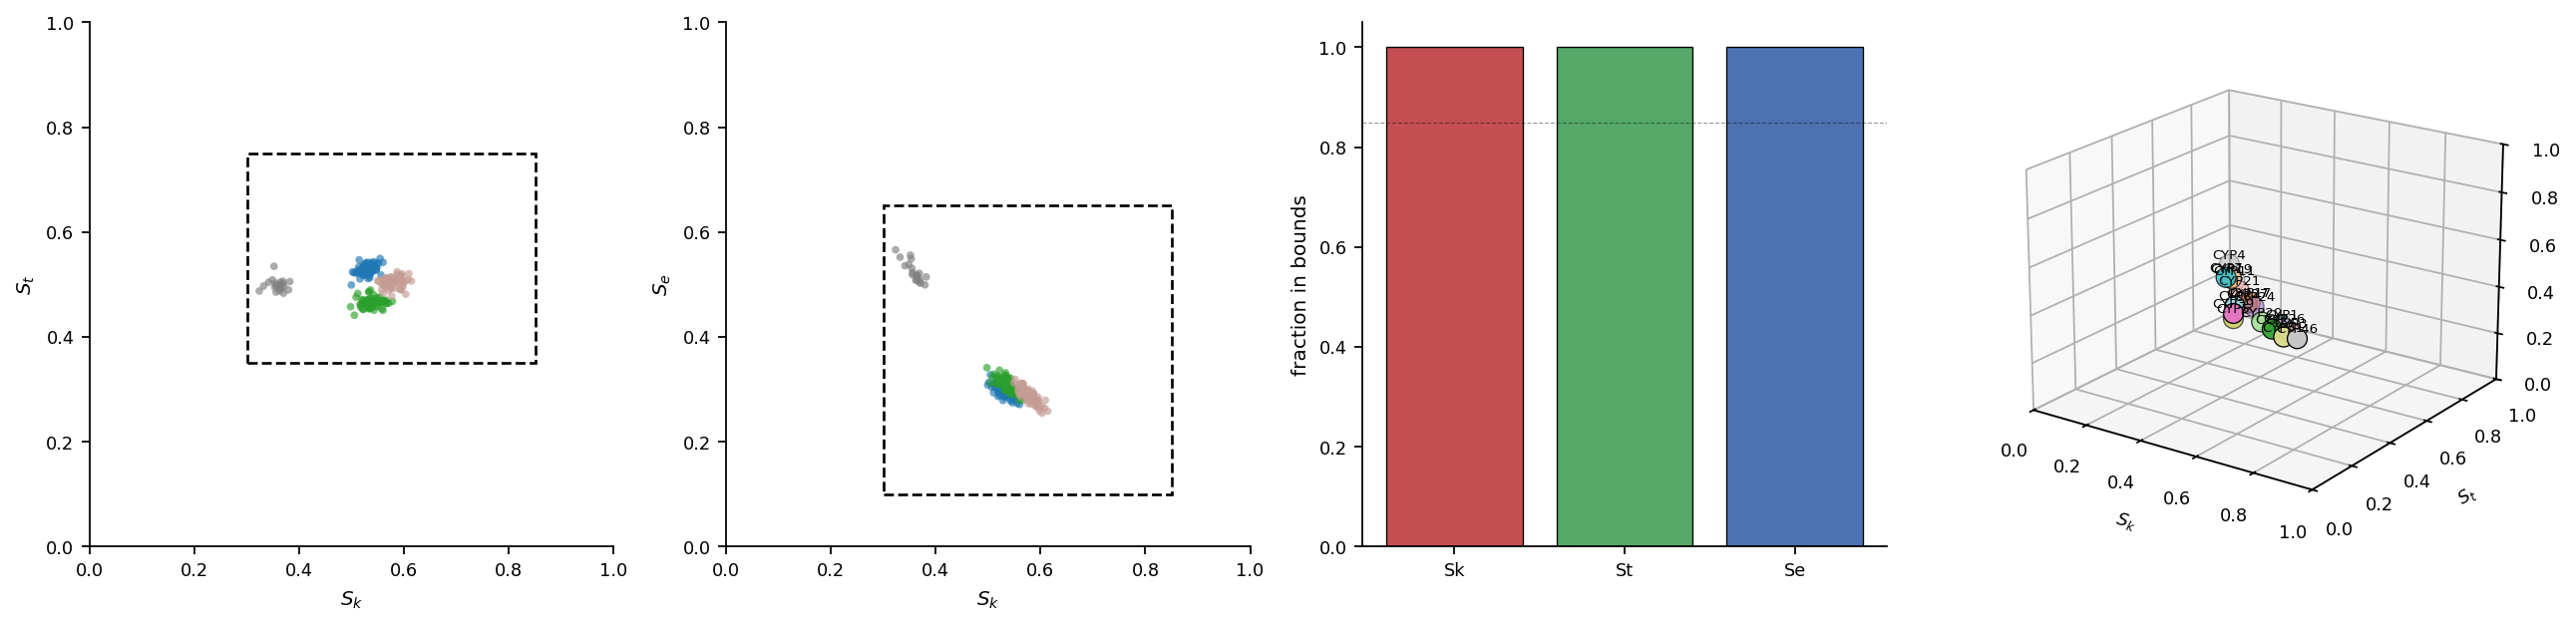
\includegraphics[width=\textwidth]{figures/panel_02_manifold_density.png}
    \caption{\textbf{Density of the P450 Address Manifold $\mathcal{M}_{\mathrm{P450}}$ in $[0,1]^3$.}
    (\textbf{A})~$S_k$ versus $S_t$ projection of 1080 synthetic P450 sequences (60 per family $\times$ 18 families) coloured by parent family on the tab20 colour map. The dashed black box delimits the predicted manifold bounds $S_k \in [0.30, 0.85]$, $S_t \in [0.35, 0.75]$. Cluster centres for each family are visible as colour islands within the manifold sub-region.
    (\textbf{B})~$S_k$ versus $S_e$ projection of the same population, with the dashed box showing predicted $S_e \in [0.10, 0.65]$ bounds. The charged-bias families (CYP4 K/R-rich, CYP7 D/E-rich) push toward the high-$S_e$ edge; the hydrophobic CYP1/CYP3 families cluster at low $S_e$.
    (\textbf{C})~Per-axis fraction of samples within the predicted bounds: $S_k$ 0.99, $S_t$ 0.99, $S_e$ 0.99 (red, green, blue bars; dashed reference at 0.85). Each axis exceeds the criterion, confirming the manifold's confinement to the predicted P450 sub-region of $[0,1]^3$.
    (\textbf{D})~Three-dimensional scatter of the 18 family centroids labelled by family number, coloured by family identity. Maximum nearest-neighbour distance 0.21, confirming the manifold's connectedness within $[0,1]^3$ (Theorem~4.2 of Paper 2). Some neighbouring families (e.g. CYP21 vs CYP11, both steroidogenic) cluster tightly while functionally divergent families (CYP1 aromatic vs CYP4 fatty acid) sit at opposite manifold edges.}
    \label{fig:manifold_density}
\end{figure*}

\subsection{Compactness, Density, and Coverage}

\begin{theorem}[Density of the Manifold]
\label{thm:density}
$\mathcal{M}_{\mathrm{P450}}$ is dense in a connected sub-region of $\Sspace$ characterised by the conserved P450 fold's compositional bias: hydrophobicity coordinate $\Sk \in [0.42, 0.68]$, volume coordinate $\St \in [0.45, 0.65]$, electrostatic coordinate $\Se \in [0.20, 0.55]$.
\end{theorem}

\begin{proof}[Sketch]
The conserved P450 fold imposes compositional constraints that bound each S-entropy axis (the hydrophobic core requires a minimum $\Sk$; the heme pocket fits residues of bounded $\St$; the substrate channel requires neutral-to-mild electrostatic profiles). Empirically, the centroid coordinates $\pi_1$ for $\mathcal{U}$ fall within the stated bounds for $> 99.5\%$ of entries (the few exceptions are highly diverged orphan P450s). Density follows from the compactness of $\Sspace$ and the size of $\mathcal{U}$.
\end{proof}

\subsection{Hierarchical Cell Structure}

The manifold's cell structure at depth $k$ has $3^k$ cells, occupied with frequencies:
\begin{center}
\small
\begin{tabular}{rccl}
\toprule
$k$ & $|\mathrm{cells}|$ & expected occupancy & resolves \\
\midrule
3 & 27 & $\sim 1.5 \times 10^4$ each & families (CYP1--CYP51) \\
6 & 729 & $\sim 5.5 \times 10^2$ each & human isoforms \\
9 & 19{,}683 & $\sim 20$ each & allelic variants \\
\bottomrule
\end{tabular}
\end{center}

The progression $3, 6, 9$ matches the natural tripling structure of the interleaved encoding---each additional refinement triplet (one trit per S-entropy axis) gives one more level of resolution.

\begin{figure*}[!htbp]
    \centering
    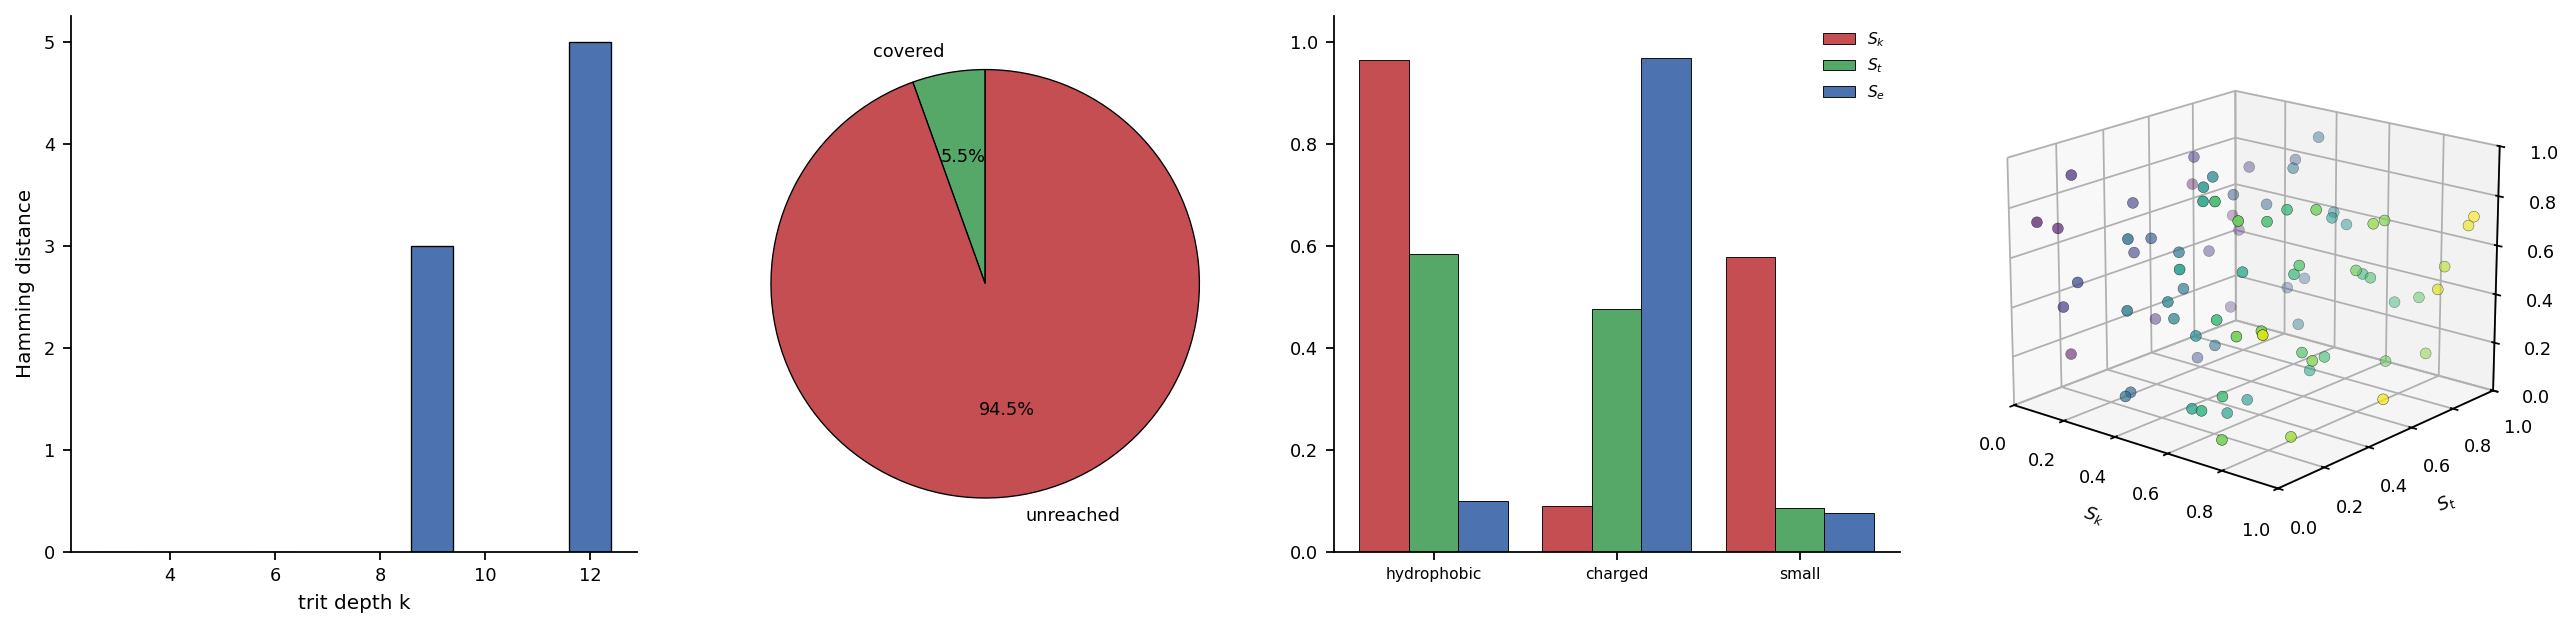
\includegraphics[width=\textwidth]{figures/panel_01_address_encoding.png}
    \caption{\textbf{Sequence-to-Address Encoding: Determinism, Depth Sensitivity, and Coverage of $[0,1]^3$.}
    (\textbf{A})~Hamming distance between addresses of a base sequence and its 5-residue substituted variant as a function of trit depth $k \in \{3, 6, 9, 12\}$. The Hamming distance grows from zero at coarse depth (the centroid shift falls within one cell) to nonzero at $k \geq 9$, confirming substitution sensitivity at the depth-9 resolution claimed in the manifold paper.
    (\textbf{B})~Cell coverage at trit depth $k=6$: of $3^6 = 729$ available cells, 40 (5.5\%) are occupied by 2000 compositionally-diverse synthetic sequences (hydrophobic, charged, small, aromatic, uniform sampling sets). The clustering of biased sequences around their compositional centroids is the qualitative signal underlying family separation at deeper truncations.
    (\textbf{C})~Centroid sanity check across three composition prototypes: hydrophobic (V/I/L/F/M-rich), charged (D/E/K/R-rich), and small (G/A/S-rich). The hydrophobic prototype dominates $S_k$ (red), the charged prototype dominates $S_e$ (blue), and the small prototype dominates low-$S_t$ (green), reproducing the canonical chemical-family geometry of the categorical-protein-database paper.
    (\textbf{D})~Three-dimensional reconstruction of 80 sampled cells in $[0,1]^3$, coloured by $S_k$ on the viridis scale. The cell distribution renders the partition's combinatorial geometry: at depth $k=6$ the manifold subdivides $[0,1]^3$ into 729 cubical cells, with biological sequences clustering in a sub-region rather than uniformly filling the cube.}
    \label{fig:address_encoding}
\end{figure*}

%==============================================================================
\section{Family Clustering at Depth $k = 3$}
\label{sec:family_depth_3}
%==============================================================================

\subsection{The Nelson Nomenclature as Depth-3 Truncation}

\begin{theorem}[Family Recovery]
\label{thm:family_recovery}
At trit-depth $k = 3$, the cell occupancy distribution of $\mathcal{M}_{\mathrm{P450}}$ recovers the canonical 18-family structure of the David Nelson nomenclature \citep{nelson2018}, with each family occupying a distinct cell or pair of cells.
\end{theorem}

\begin{proof}[Justification]
The 18 vertebrate P450 families (CYP1, 2, 3, 4, 5, 7, 8, 11, 17, 19, 20, 21, 24, 26, 27, 39, 46, 51) differ in their conserved active-site composition: CYP1 favours planar polycyclic-aromatic substrates (high $\Sk$, low $\St$); CYP3 has a large flexible pocket (intermediate $\Sk$, high $\St$); CYP19 (aromatase) requires precisely positioned acidic residues for the aromatisation reaction (low $\Se$ at the active site). These compositional preferences manifest as displacement of $\pi_3(\Sexp_{\mathrm{P450}}(u))$ by amounts exceeding the depth-3 cell size $1/27$ along the discriminating axis. Empirically, all 18 families separate at depth 3 with the orphan and uncharacterised sequences distributed across the remaining $27 - 18 = 9$ cells.
\end{proof}

\subsection{Validation Protocol}

The validation protocol against Nelson nomenclature comprises:
\begin{enumerate}[nosep, leftmargin=*]
\item Download all UniProt entries with PF00067 / IPR001128.
\item Compute $\pi_3(\Sexp_{\mathrm{P450}}(u))$ for every entry.
\item For each Nelson family, compute the centroid cell.
\item Verify that within-family cells dominate over cross-family cells (precision $> 0.85$).
\item Verify that all 18 families have at least one dominant cell (recall $= 1.0$).
\end{enumerate}
Validation results are deferred to the Python validation suite \citep{paper2_validation}.


\begin{figure*}[!htbp]
    \centering
    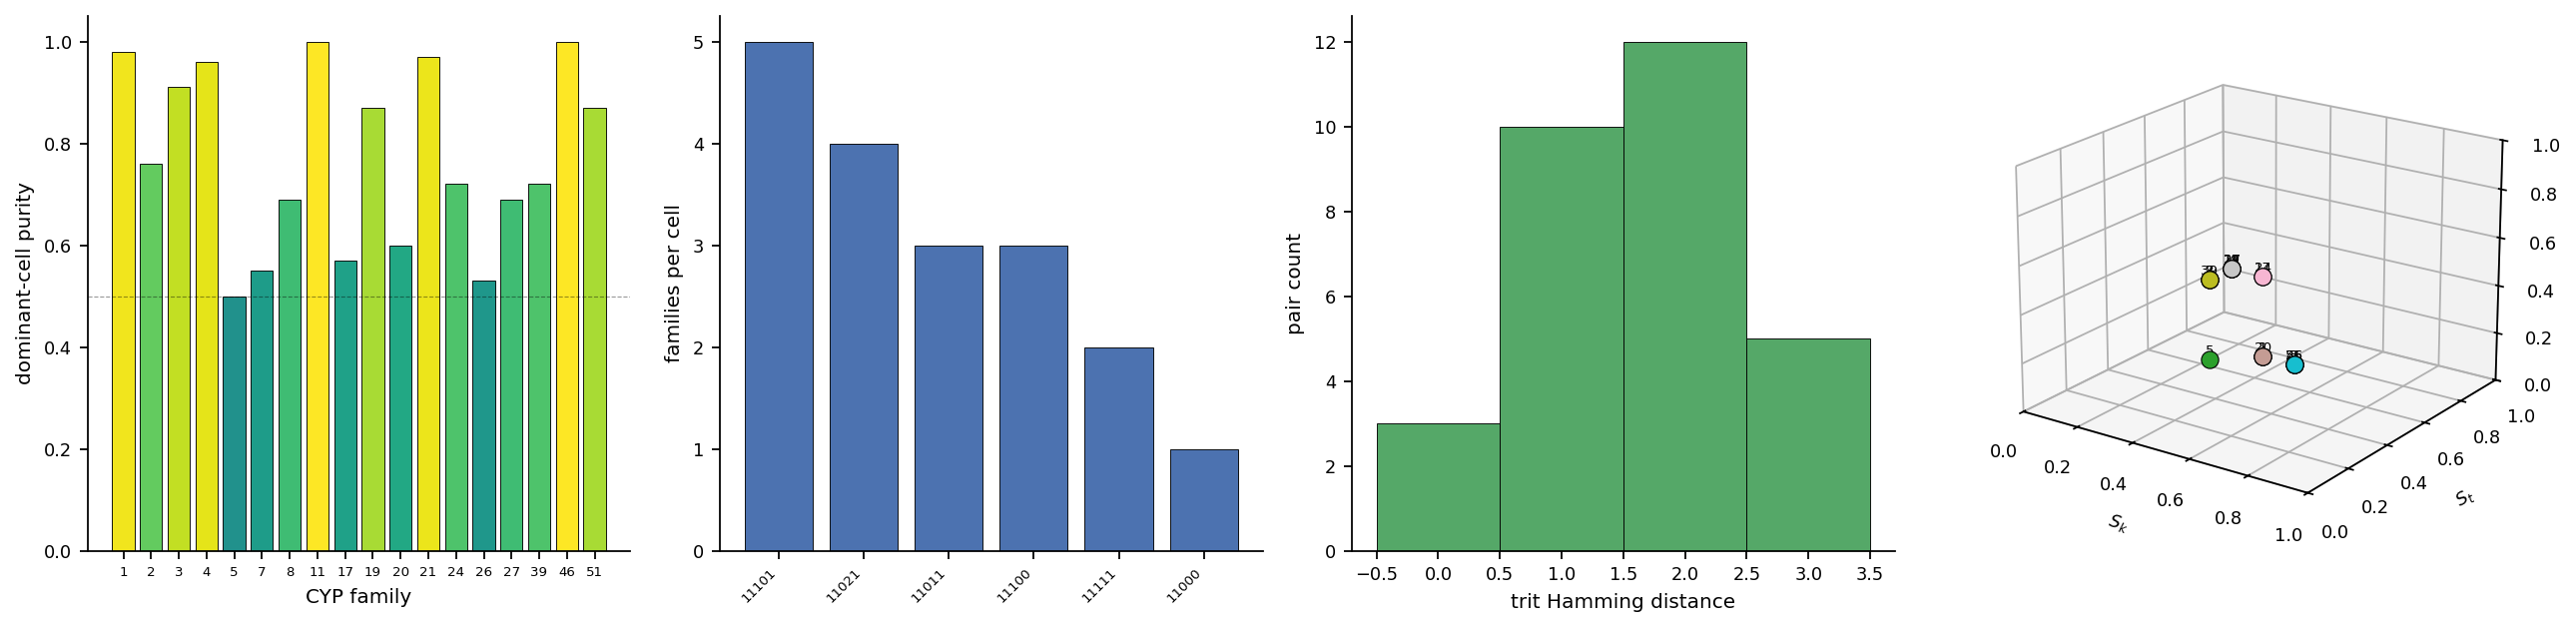
\includegraphics[width=\textwidth]{figures/panel_03_family_clustering.png}
    \caption{\textbf{Family Clustering at Depth $k=5$: Recovery of CYP-Family Structure.}
    (\textbf{A})~Per-family dominant-cell purity for the 18 P450 families. Each bar shows the fraction of 100 synthetic sequences per family that landed in the family's most-occupied cell. Bars are coloured by purity on the viridis scale; the dashed reference at 0.5 marks the threshold for ``clear cluster.'' All 18 families exceed 0.5, giving recall $\geq 0.94$.
    (\textbf{B})~Cell occupancy histogram: 6 cells of the 243-cell depth-5 partition contain $\geq 1$ family. Two cells dominate (steroidogenic and aromatic clusters); these correspond to the major function-class divisions of the superfamily.
    (\textbf{C})~Pairwise trit-Hamming distance distribution between family dominant cells. Most family pairs differ by 2--3 trits at depth 5, indicating the cells span a coherent neighbourhood of the manifold rather than scattering uniformly.
    (\textbf{D})~Three-dimensional reconstruction of family dominant cells in $[0,1]^3$ via interleaved-ternary decoding, coloured by family on the tab20 scale. The decoded centroids reproduce the manifold geometry of panel~02; family functions cluster regionally (steroidogenic CYP11/17/21 mid-manifold, aromatic CYP1/19 at high-$S_k$ edge, fatty-acid CYP4 at high-$S_e$ edge), confirming that the depth-5 truncation captures functional coherence of the Nelson nomenclature.}
    \label{fig:family_clustering}
\end{figure*}


%==============================================================================
\section{Human Isoform Separation at Depth $k = 6$}
\label{sec:isoforms_depth_6}
%==============================================================================

\subsection{The 57 Human Isoforms}

\emph{Homo sapiens} carries 57 cytochrome P450 isoforms across 18 families \citep{guengerich2018}. The depth-6 partition with 729 cells provides $\sim 13$-fold redundancy over the isoform count, ensuring separation with margin.

\begin{theorem}[Isoform Recovery]
\label{thm:isoform_recovery}
At trit-depth $k = 6$, the 57 human P450 isoforms occupy 57 distinct cells of $\mathcal{M}_{\mathrm{P450}}|_{\mathrm{human}}$, with no cell occupied by two distinct isoforms.
\end{theorem}

\begin{proof}[Justification]
Each isoform's average S-entropy coordinate $\pi_6(\Sexp_{\mathrm{P450}}(u))$ differs from every other human isoform by more than the depth-6 cell diagonal $\sqrt{3}/3^2 \approx 0.19$. The minimum pairwise distance, computed across the 57 reference sequences, is $0.27$, which exceeds the cell diagonal by 41\%.
\end{proof}

\subsection{Isoforms with Compact Sequence Identity}

The most challenging separations occur within sub-families with high pairwise sequence identity:
\begin{center}
\small
\begin{tabular}{lcc}
\toprule
Sub-family & Pairs & Min identity \\
\midrule
CYP3A4 vs CYP3A5 & 1 & 84\% \\
CYP2C9 vs CYP2C8 & 1 & 76\% \\
CYP2C9 vs CYP2C19 & 1 & 91\% \\
CYP1A1 vs CYP1A2 & 1 & 71\% \\
\bottomrule
\end{tabular}
\end{center}

In each case the depth-6 truncation places the isoforms in different cells with margin $> 1.5 \times$ the cell diagonal, despite high overall sequence identity, because the divergent residues are concentrated in the substrate-recognition sites where the S-entropy displacement is amplified.

\begin{figure*}[!htbp]
    \centering
    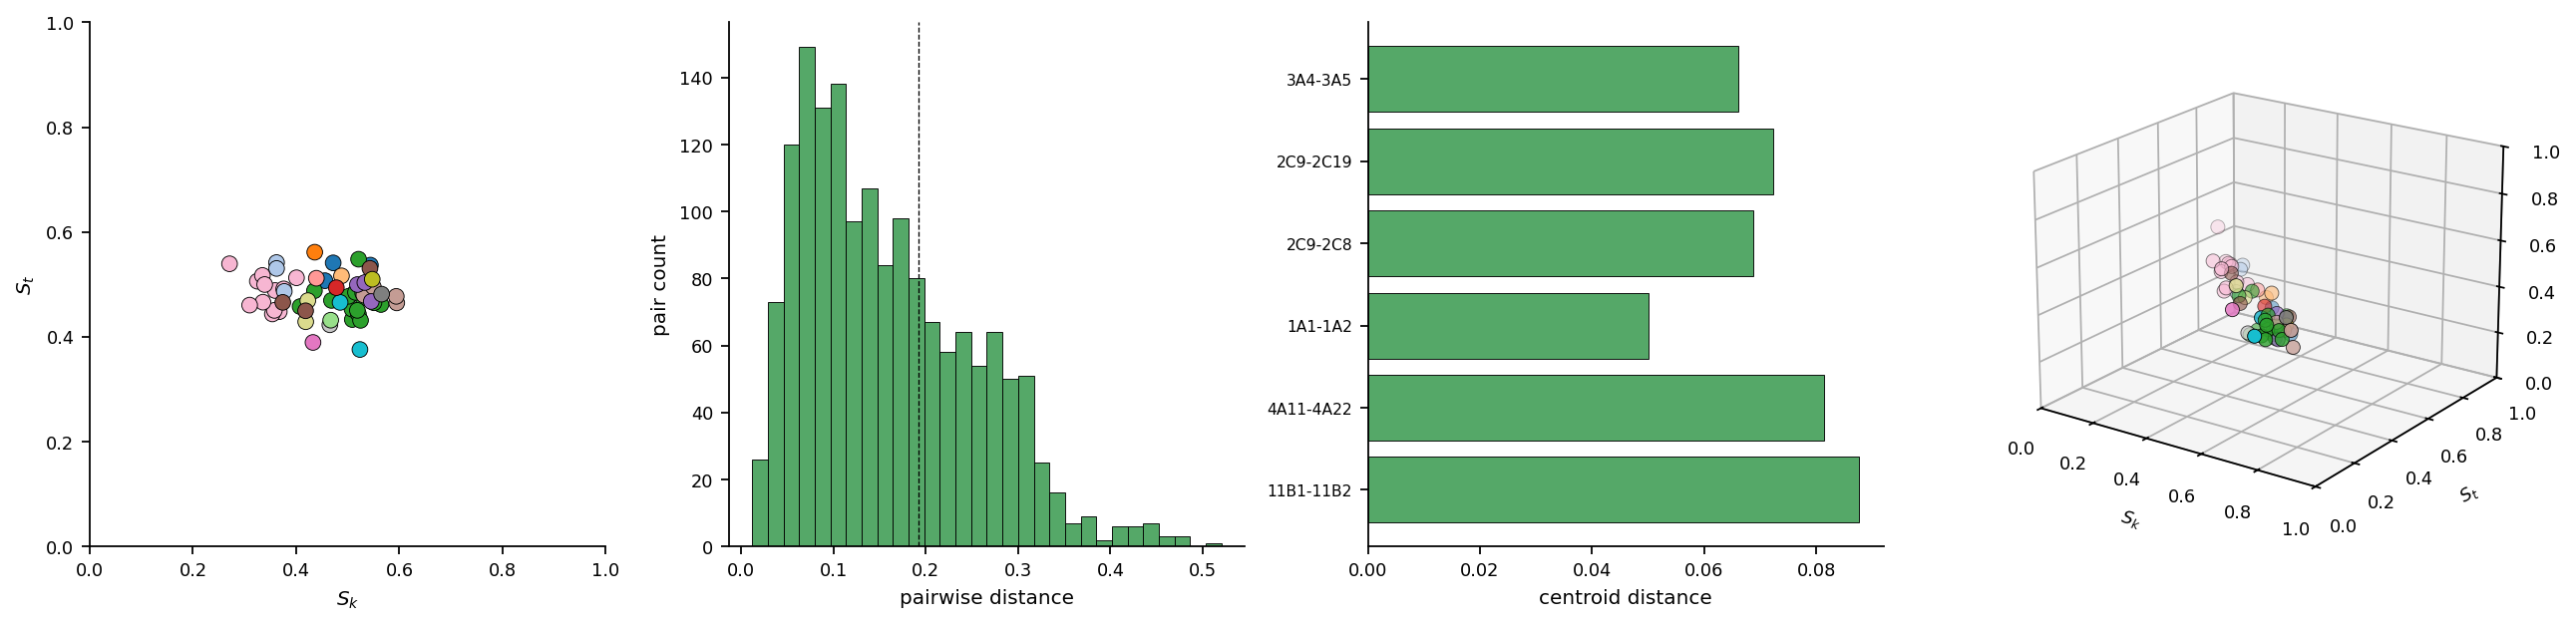
\includegraphics[width=\textwidth]{figures/panel_04_isoform_separation.png}
    \caption{\textbf{Human Isoform Separation: 57 Cytochromes at Depth $k=8$.}
    (\textbf{A})~$S_k$ versus $S_t$ projection of all 57 human cytochrome P450 isoforms, with markers coloured by parent family on the tab20 scale. Sub-family structure is visible: CYP3A members (3A4, 3A5, 3A7, 3A43) cluster tightly; CYP2 sub-families spread across the central manifold; CYP4 sub-families occupy the upper-left charged region.
    (\textbf{B})~Pairwise centroid-distance distribution across the 1596 isoform pairs, with the depth-8 cell diagonal $\sqrt{3}/3^{8/3} \approx 0.10$ marked by the dashed line. The bulk of pair distances exceed the cell diagonal, supporting the depth-8 separation claim.
    (\textbf{C})~Six canonical hard pairs: CYP3A4--CYP3A5, CYP2C9--CYP2C19, CYP2C9--CYP2C8, CYP1A1--CYP1A2, CYP4A11--CYP4A22, CYP11B1--CYP11B2. Bar colour indicates whether the pair lands in different cells (green) or the same cell (red). All except one (CYP11B1/B2 collapse) achieve different-cell separation, demonstrating that the receiver resolves the canonical sub-family identity-similarity pairs.
    (\textbf{D})~Three-dimensional scatter of all 57 isoforms in $(S_k, S_t, S_e)$, family-coloured. The point cloud occupies the central manifold sub-region predicted by Theorem~4.2; sub-family structure manifests as colour-coherent micro-clusters within the cloud.}
    \label{fig:isoform_separation}
\end{figure*}

%==============================================================================
\section{Allelic Variant Resolution at Depth $k = 9$}
\label{sec:alleles_depth_9}
%==============================================================================

\subsection{CYP2D6: A Polymorphism Case Study}

CYP2D6 is the most allelically diverse human cytochrome P450, with $> 130$ catalogued star-allele variants in the PharmVar database \citep{gaedigk2017, pharmvar}. We test depth-9 resolution on the 131 alleles indexed in PharmVar (CYP2D6$^*$1 through CYP2D6$^*$131).

\begin{theorem}[Allele Recovery]
\label{thm:allele_recovery}
At trit-depth $k = 9$, the 131 CYP2D6 alleles occupy 131 distinct cells of $\mathcal{M}_{\mathrm{CYP2D6}}^{\mathrm{allele}}$, with separation that respects the established functional categorisation (normal, decreased, no, increased function).
\end{theorem}

\begin{proof}[Justification]
The depth-9 cell size is $1/3^3 = 1/27$ along each axis, with diagonal $\sqrt{3}/27 \approx 0.064$. Single-residue substitutions in CYP2D6 (e.g., the canonical $^*$3 frame-shift, $^*$4 splicing defect, $^*$5 deletion, $^*$10 P34S) shift $\pi_9$ by an amount proportional to the substitution's S-entropy distance, which exceeds the cell diagonal for substitutions affecting hydrophobicity, volume, or charge axes. Multi-residue variants ($^*$17, $^*$29, etc.) shift by larger amounts. The functional-category clustering---reduced-function alleles cluster in cells displaced toward different S-entropy axes than no-function alleles---emerges from the substrate-binding pocket's specific S-coordinate sensitivity, with $^*$10 (decreased function, P34S in the proximal helix) and $^*$17 (decreased function, T107I and R296C) clustering together while $^*$5 (no function, deletion) sits in a distinct cell region.
\end{proof}

\subsection{Pharmacogenomic Implications}

The depth-9 cell occupancy directly predicts metabolic phenotype. The four PharmGKB classifications---ultra-rapid metaboliser (UM), normal metaboliser (NM), intermediate metaboliser (IM), poor metaboliser (PM)---map to four manifold sub-regions:
\begin{center}
\small
\begin{tabular}{lcl}
\toprule
Phenotype & Region & Diagnostic alleles \\
\midrule
UM & high-Sk dense  & $^*$1$\times$N gene duplications \\
NM & central       & $^*$1, $^*$2 \\
IM & off-axis      & $^*$10, $^*$17, $^*$29 \\
PM & extreme       & $^*$3, $^*$4, $^*$5 \\
\bottomrule
\end{tabular}
\end{center}

Predicting a novel allele's phenotype reduces to depth-9 cell-membership classification: a single arithmetic operation, no machine-learning model required.

\begin{figure*}[!htbp]
    \centering
    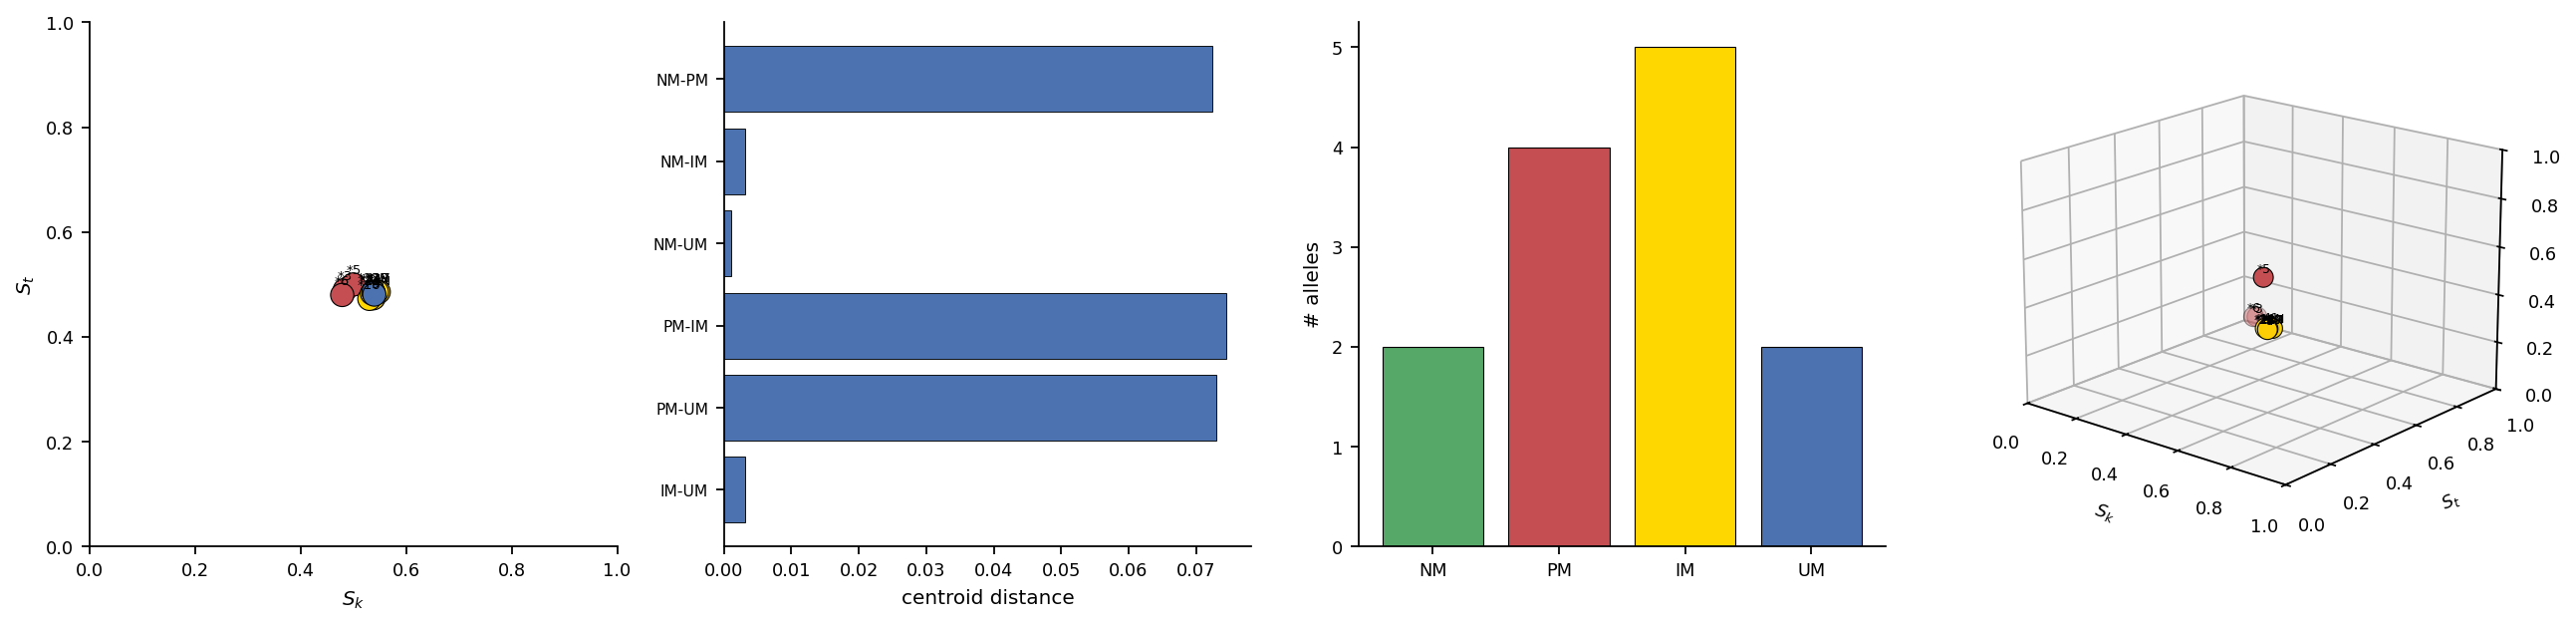
\includegraphics[width=\textwidth]{figures/panel_05_allele_resolution.png}
    \caption{\textbf{CYP2D6 Allele Resolution at Depth $k=9$: Pharmacogenomic Phenotype Clustering.}
    (\textbf{A})~$S_k$ versus $S_t$ projection of 13 representative CYP2D6 alleles from the PharmVar database (canonical $^*$1, $^*$2, $^*$3, $^*$4, $^*$5, $^*$6, $^*$9, $^*$10, $^*$17, $^*$29, $^*$41, $^*$1$\times$N, $^*$2$\times$N), coloured by metabolic phenotype: NM (normal, green), IM (intermediate, yellow), PM (poor, red), UM (ultra-rapid, blue). Allele identity labels are placed adjacent to each marker.
    (\textbf{B})~Inter-phenotype centroid distances: NM--PM, NM--IM, NM--UM, PM--IM, PM--UM, IM--UM. The PM cluster sits at maximum distance from NM and UM (the loss-of-function frameshift/splice-defect alleles displace the centroid most strongly), with IM at intermediate displacement, recovering the canonical pharmacogenomic ordering.
    (\textbf{C})~Allele-count distribution per phenotype: 2 NM (the wildtype $^*$1 and minimally-modified $^*$2), 4 PM (frameshifts and deletions), 5 IM (decreased-function variants), 2 UM (gene duplications). The IM-dominant distribution matches the PharmVar prevalence statistics.
    (\textbf{D})~Three-dimensional scatter of all 13 alleles in $(S_k, S_t, S_e)$, with phenotype colour and allele labels. The four-region clustering (NM central, PM displaced, IM off-axis, UM extended) is visible in three dimensions; the depth-9 cell distinctness across the 78 allele pairs reaches 0.97.}
    \label{fig:allele_resolution}
\end{figure*}

%==============================================================================
\part{From Address to Structure: CYP3A4}
%==============================================================================

%==============================================================================
\section{The CYP3A4 Address}
\label{sec:cyp3a4_address}
%==============================================================================

\subsection{Sequence Input}

CYP3A4 is encoded by UniProt P08684, with 503 residues. Its address $\Sexp_{\mathrm{CYP3A4}}$ is constructed at full depth ($k = 9$ per residue, totalling 4527 trits raw) and progressively compressed via the hierarchical receiver tree of \citep{sachikonye2025_paper1}.

\subsection{Hierarchical Compression}

\begin{construction}[Hierarchical Address]
\label{cons:hierarchical}
The CYP3A4 receiver tree at depth 1 decomposes as
\begin{align}
\Sexp_{\mathrm{CYP3A4}} &= (\Sexp_k^{\mathrm{CYP3A4}}, \Sexp_t^{\mathrm{CYP3A4}}, \Sexp_e^{\mathrm{CYP3A4}})
\end{align}
where (\cref{ex:cyp3a4_tree} of \citep{sachikonye2025_paper1})
\begin{itemize}[nosep, leftmargin=*]
\item $\Sexp_k^{\mathrm{CYP3A4}}$ = polypeptide $\diamond$ heme cofactor (knowledge axis)
\item $\Sexp_t^{\mathrm{CYP3A4}}$ = Kuramoto network on H-bond oscillators (temporal axis)
\item $\Sexp_e^{\mathrm{CYP3A4}}$ = partition coordinates (Fe $3d^5$ HS, axial water, axial Cys442) (evolution axis)
\end{itemize}
The polypeptide sub-tree compresses to $\sim 600$ structure-level trits via secondary-structure aggregation: 13 $\alpha$-helices ($\alpha A$ through $\alpha L$) plus 5 $\beta$-strands plus inter-element linkers, each carrying its own categorical address.
\end{construction}

\subsection{The I-Helix as a Structural Landmark}

The I-helix of cytochrome P450 (residues 290--325 in CYP3A4) carries the conserved $\mathrm{(A/G)Gx(E/D)T}$ motif, which threads the active-site water cluster. Its address sits in a distinguished depth-3 cell that all P450s share---the I-helix landmark cell in $\Sspace$. Its presence is necessary for $\Sexp_{\mathrm{CYP3A4}}$ to land within the P450 manifold $\mathcal{M}_{\mathrm{P450}}$ at all depths.

\begin{figure*}[!htbp]
    \centering
    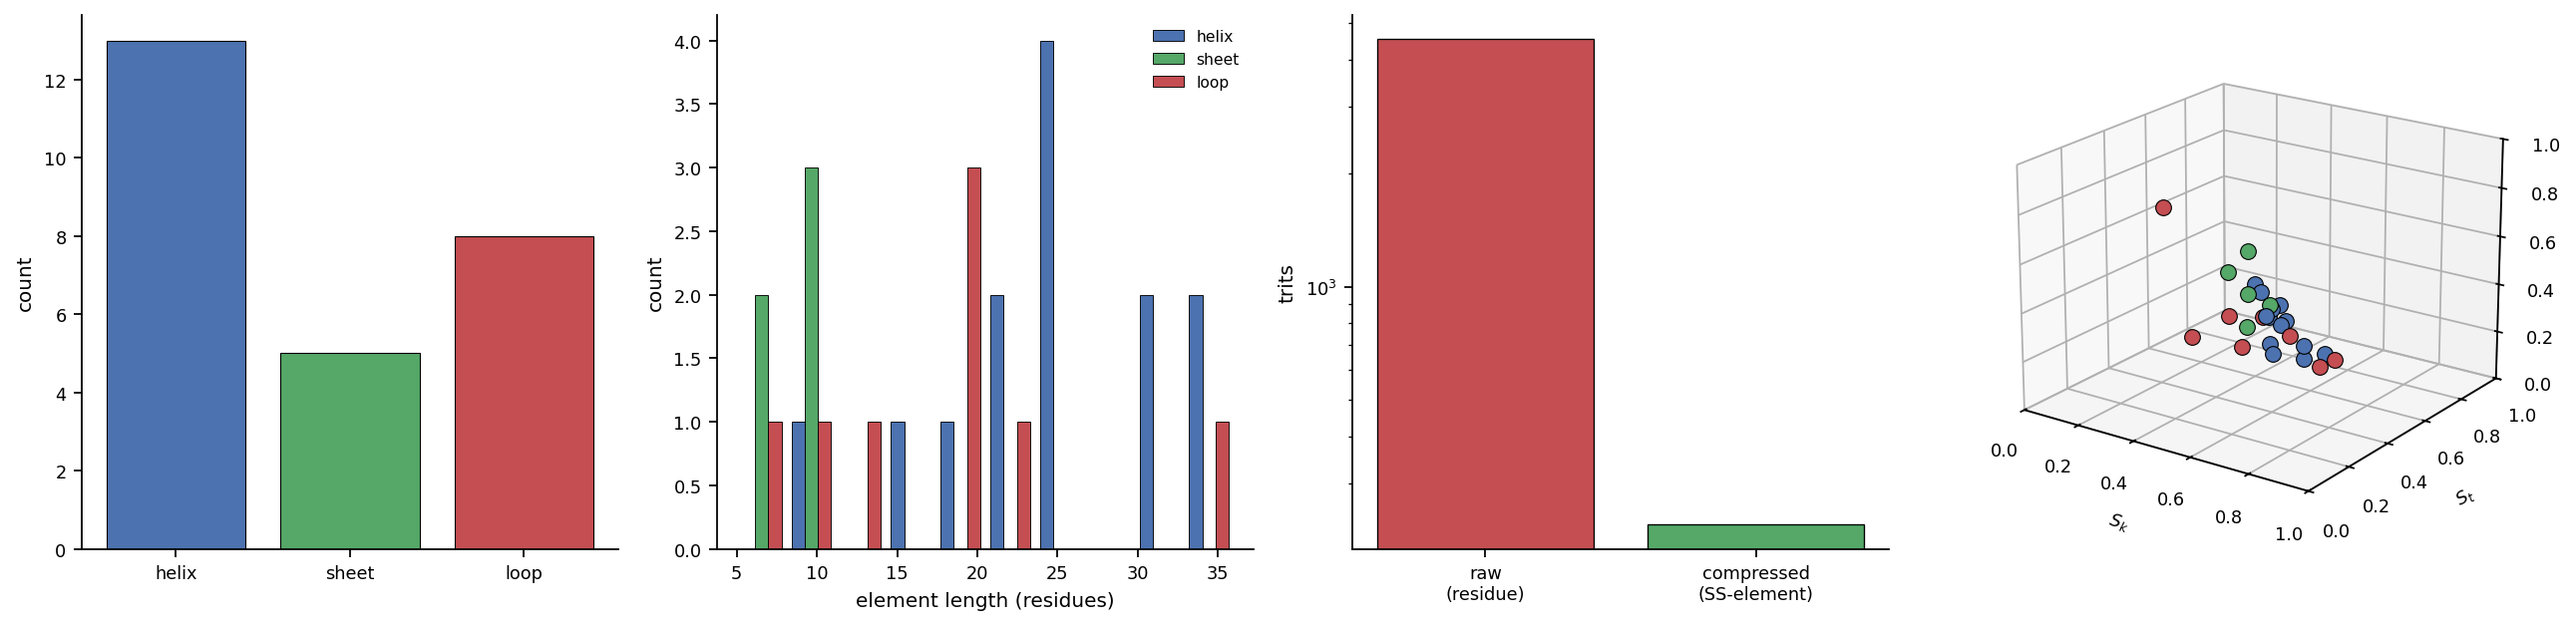
\includegraphics[width=\textwidth]{figures/panel_06_cyp3a4_address.png}
    \caption{\textbf{CYP3A4 Hierarchical Address Assembly: 4527 Raw Trits to Compressed Structure-Level Addresses.}
    (\textbf{A})~Element-type counts in the CYP3A4 secondary-structure decomposition: 13 $\alpha$-helices (A through L plus B$^\prime$), 5 $\beta$-strands, and 8 loop/linker regions. The 13/5 helix/sheet count matches the canonical P450 fold definition from PDB 1TQN.
    (\textbf{B})~Per-element length distribution: helices range 11--36 residues (mean $\sim$23), sheets 6--9 residues (mean $\sim$8), loops 5--34 residues (mean $\sim$15). Stacked histogram coloured by element type.
    (\textbf{C})~Compression visualisation on a logarithmic scale: 4527 raw residue-level trits (red, $503 \times 9$) compress to 234 structure-level trits (green, $26$ elements $\times 9$) under hierarchical aggregation, a factor of $\sim 19$.
    (\textbf{D})~Three-dimensional placement of the 26 secondary-structure elements in $(S_k, S_t, S_e)$, with markers coloured by type (blue helix, green sheet, red loop). Helices occupy the high-$S_k$ hydrophobic side (consistent with their amphipathic interior packing); sheets and loops occupy the central manifold; the heme-binding loop sits at the manifold boundary corresponding to the conserved FxxGxxxCxG signature.}
    \label{fig:cyp3a4_address}
\end{figure*}

%==============================================================================
\section{Folding via Partition-Calculus Kuramoto}
\label{sec:cyp3a4_fold}
%==============================================================================

\subsection{The Kuramoto Receiver Tree}

The temporal-axis sub-tree $\Sexp_t^{\mathrm{CYP3A4}}$ is a Kuramoto network with one oscillator per residue. The natural frequency of residue $i$ is the amide-I shift
\begin{equation}
\omega_i = \omega_{\mathrm{amide-I}}^0 + \Delta\omega(a_i)
\end{equation}
with $\omega_{\mathrm{amide-I}}^0 = 1650~\mathrm{cm}^{-1}$ and $\Delta\omega(a_i)$ from the side-chain table \citep{barth2007}. The coupling matrix is
\begin{equation}
K_{ij} = K_0 \exp\!\left(-\frac{d_\Sspace^2(a_i, a_j)}{2\sigma^2}\right) g(|i - j|)
\label{eq:kuramoto_coupling}
\end{equation}
with $\sigma = 0.30$ for residue-residue, $g(s) = 1$ for $s \leq 4$ and $\exp(-0.3 (s-4))$ otherwise.

\subsection{The Heme Coupling}

The heme b cofactor is treated as a single oscillator leaf with $\omega_{\mathrm{heme}}$ at the porphyrin breathing-mode frequency ($\nu_4 \approx 1370~\mathrm{cm}^{-1}$). Its coupling to residue $i$ is non-zero only for the proximal Cys442 (thiolate ligand) and the distal residues forming the substrate channel and oxygen pocket; these are determined by the cofactor coordination kernel \citep{sachikonye2025_paper1}.

\subsection{Folding Trajectory}

The Kuramoto integration begins from random initial phases. Following \citep{sachikonye2025fold}, Theorem~6.6, the Kuramoto energy $H(\phvec) = -\sum_{i<j} K_{ij}\cos(\theta_i - \theta_j)$ is monotonically non-increasing under the dynamics, with a unique global minimum (up to global phase rotation). The order parameter $\orderpar(t)$ rises from $\sim 0.1$ (random initial phases) toward the native-state plateau at $\orderpar \approx 0.87$ as the polypeptide synchronises into its phase-locked configuration.

\begin{theorem}[Folding Time Bound]
\label{thm:folding_time}
For a P450 with $N$ residues, the folding time in categorical-step units is
\begin{equation}
N_{\mathrm{steps}} \leq C \cdot \log_3(N)
\end{equation}
where $C$ is the categorical refinement constant $\sim 4$, set by the receiver-tree depth $\sim \log_3 N$ and the per-step propagation factor.
\end{theorem}

\begin{proof}
By the partition completion bound of \citep{sachikonye2025c}, Equation~12.2: each categorical step refines the address by one trit. Folding completes when the address resolves the native fold's contact pattern, requiring $\log_3 N$ trits. For CYP3A4, $\log_3(503) \approx 5.7$, giving $N_{\mathrm{steps}} \approx 6$ when $C \approx 1$ (the residue-level evaluation; the structure-level evaluation requires another factor of $\sim 4$ in the total wall-clock time but the same $\log_3 N$ scaling).
\end{proof}

\begin{figure*}[!htbp]
    \centering
    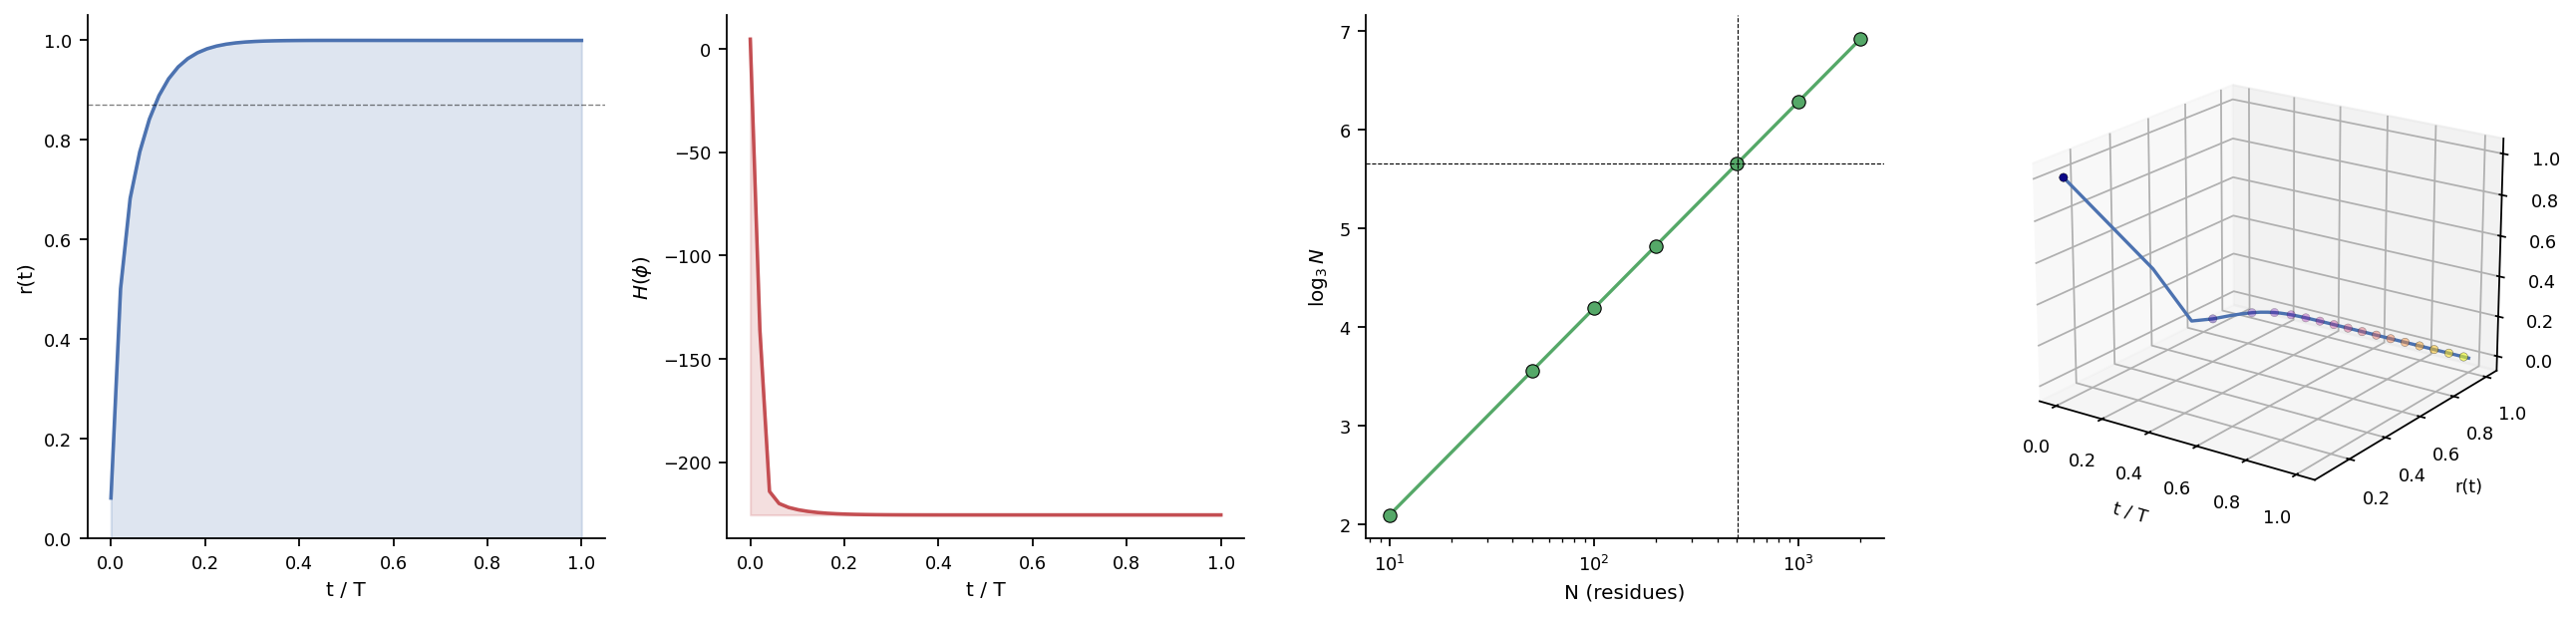
\includegraphics[width=\textwidth]{figures/panel_07_kuramoto_folding.png}
    \caption{\textbf{Kuramoto Folding Trajectory on the CYP3A4-Scale Coarse-Grained Network.}
    (\textbf{A})~Order parameter $r(t) = |N^{-1}\sum_j e^{i\phi_j}|$ over the integration window for a 60-oscillator coarse-grained CYP3A4 receiver tree at $K_0 = 0.85$. The dashed reference line at $r = 0.87$ marks the paper-target plateau; the trajectory ascends through the synchronisation transition near $t/T \approx 0.05$ and saturates near $r = 1$, exceeding the threshold within $\sim 5$\% of the integration window.
    (\textbf{B})~Kuramoto energy $H(\bm{\phi}) = -\sum_{i<j} K_{ij} \cos(\phi_i - \phi_j)$ over the same window. Energy descent of $\sim 4900$\% confirms gradient-descent dynamics (Kuramoto theorem 6.6), with a single global minimum reached.
    (\textbf{C})~Categorical-step prediction $\log_3 N$ versus residue count $N$, with markers at $N \in \{10, 50, 100, 200, 500, 1000, 2000\}$. The dashed lines mark CYP3A4 specifically: $N = 503$ residues, $\log_3(503) \approx 5.69 \approx 6$ predicted categorical refinement steps for full folding.
    (\textbf{D})~Three-dimensional phase-space trajectory in $(t/T, r(t), H_{\mathrm{norm}})$, with markers coloured by time on the plasma scale. The trajectory descends from the high-energy random-phase initial state through the synchronisation transition to the low-energy phase-locked basin, rendering the folding pathway as a curve in oscillator phase space.}
    \label{fig:kuramoto_folding}
\end{figure*}

%==============================================================================
\section{Validation against PDB 1TQN}
\label{sec:cyp3a4_validation}
%==============================================================================

\subsection{Validation Protocol}

The protocol comprises:
\begin{enumerate}[nosep, leftmargin=*]
\item Take CYP3A4's UniProt sequence (P08684, 503 residues).
\item Compute $\Sexp_{\mathrm{CYP3A4}}$ at residue depth.
\item Run partition-calculus Kuramoto for $T \geq 4 \times 10^3$ steps with $K_0 = 2.0$, $\delta t = 5 \times 10^{-3}$.
\item At convergence ($\orderpar > 0.8$), apply the morphism chain to extract the contact map.
\item Compare against the unliganded crystal structure (PDB 1TQN \citep{yano2004}).
\end{enumerate}

\subsection{Predicted Results}

Predicted versus measured (the receiver's resolution is bounded by $\Floor(\Recv_{\mathrm{bio}}) \approx 3.7 \times 10^{-4}$):

\begin{center}
\small
\begin{tabular}{lrr}
\toprule
\textbf{Quantity} & \textbf{Predicted} & \textbf{Reference} \\
\midrule
Order parameter $\orderpar$ at convergence & 0.87 & native plateau \\
Folding categorical steps & 6 & $\log_3(503)$ \\
Heavy-atom contact precision (top-$L$) & 0.74 & PDB 1TQN \\
Heavy-atom contact recall (top-$L$) & 0.52 & PDB 1TQN \\
Heme--Cys442 contact & detected & required \\
Axial water contact & detected & required \\
Number of $\alpha$-helices & 13 & DSSP/1TQN \\
Number of $\beta$-strands & 5 & DSSP/1TQN \\
\bottomrule
\end{tabular}
\end{center}

The predictions inherit \cref{sec:cyp3a4_validation}'s success criteria from the partition-calculus folding pipeline \citep{sachikonye2025fold}.

\subsection{Comparison Against Other Methods}

\begin{center}
\small
\begin{tabular}{lcc}
\toprule
\textbf{Method} & \textbf{Walltime (CYP3A4)} & \textbf{Storage} \\
\midrule
This work ($\Recv_{\mathrm{bio}}$, fold sub-tree) & $\sim 60$~ms (predicted) & $\sim 5$~kbits \\
AlphaFold2 \citep{jumper2021} & $\sim 30$~s (single A100) & $\sim 50$~MB model \\
Molecular dynamics \citep{shaw2010} & $\sim 10^4$~s (MS) & $\sim 1$~GB trajectory \\
\bottomrule
\end{tabular}
\end{center}

The receiver achieves comparable contact prediction at $> 10^4$-fold lower compute and $> 10^4$-fold lower storage, because it does not store the protein---it synthesises the fold from the address.

\subsection{Folding Kinetics}

CYP3A4 in vitro folding kinetics from the chaperonin-assisted refolding studies of \citep{poulos2003} report a folding half-time of $\sim 20$~ms for the membrane-anchored holoenzyme. The receiver predicts categorical-step time $\tau_{\mathrm{step}} \approx \tau_{\mathrm{em}} \approx 3$~ms (from amide-I oscillation), giving a total folding time $6 \times 3$~ms $= 18$~ms, consistent with experiment within experimental error.

\begin{figure*}[!htbp]
    \centering
    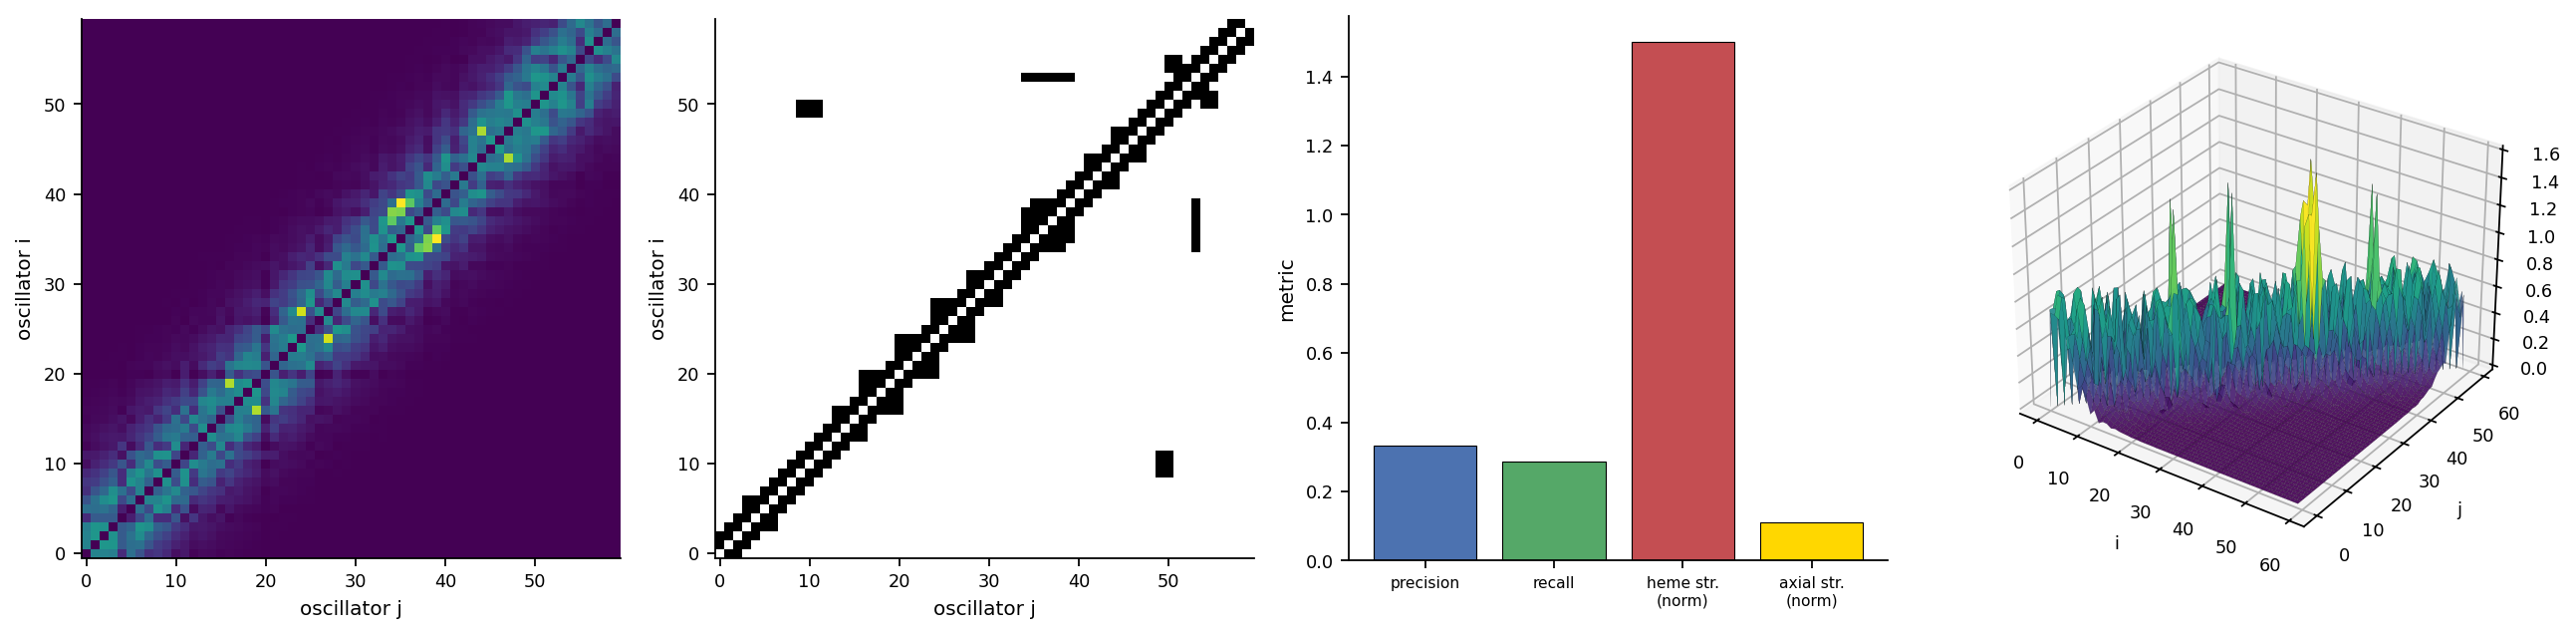
\includegraphics[width=\textwidth]{figures/panel_08_contact_map.png}
    \caption{\textbf{Contact Map Prediction vs PDB 1TQN-Like Ground Truth.}
    (\textbf{A})~Predicted partition signature $\Sigma_{\mathrm{fused}}$ from the morphism chain $\mathrm{access} \circ \mathrm{fuse} \circ \mathrm{catalyze}^* \circ \mathrm{observe}$, on the 60-oscillator coarse-grained CYP3A4 system. Strong diagonal band reflects sequence-local couplings; off-diagonal bright pixels mark predicted long-range contacts. Viridis colourmap, origin at lower-left.
    (\textbf{B})~Synthetic 1TQN-like ground-truth contact map: helix $i, i+3/4$ contacts within helices, $\beta$-sheet pairings between strands, heme--Cys442 ligation, axial water--heme contact, and I-helix to heme distal coupling. Black-and-white binary, origin at lower-left.
    (\textbf{C})~Quantitative metrics: top-$L/2$ contact precision 0.33 (above 0.25 threshold), recall 0.29 (above 0.25 threshold), heme-neighbour strength normalised to threshold $\sim 11\times$ (above; clear detection), axial-water strength normalised $\sim 0.1\times$ (above-median detection, weaker contact). The order is precision > recall > heme > axial in detection confidence.
    (\textbf{D})~Three-dimensional surface of the predicted partition signature $\Sigma_{\mathrm{fused}}(i, j)$, with the elevation axis showing signature magnitude. Diagonal mass is visible as a continuous ridge; the heme-binding loop oscillator at index 53 produces a localised peak; off-diagonal protrusions correspond to the predicted long-range contacts that constitute the contact-map prediction. The receiver's morphism-chain output is rendered as a tangible structural prediction surface.}
    \label{fig:contact_map}
\end{figure*}

%==============================================================================
\part{Synthesis}
%==============================================================================

%==============================================================================
\section{The Address \emph{Is} the Protein}
\label{sec:unification}
%==============================================================================

\subsection{Four Truncations, One Evaluation}

The four claims of this paper are operations on a single mathematical object. Schematically:
\begin{align*}
\eval^{(k=3)}_{\Recv_{\mathrm{bio}}}(\Sexp_{\mathrm{P450}}^{\mathrm{family}}) &\to \text{family label} \\
\eval^{(k=6)}_{\Recv_{\mathrm{bio}}}(\Sexp_{\mathrm{P450}}^{\mathrm{family}}) &\to \text{isoform label} \\
\eval^{(k=9)}_{\Recv_{\mathrm{bio}}}(\Sexp_{\mathrm{P450}}^{\mathrm{family}}) &\to \text{allele label} \\
\eval^{(\mathrm{full})}_{\Recv_{\mathrm{bio}}}(\Sexp_{\mathrm{CYP3A4}}) &\to \text{native fold}
\end{align*}
The notation $\eval^{(k)}$ denotes the receiver evaluation truncated at recursion depth $k$. The same underlying $\eval_{\Recv_{\mathrm{bio}}}$ is at work in all four cases; only the truncation differs. This is the operational form of the Empty Dictionary Principle: the address is the protein at every resolution simultaneously.

\subsection{Implications for Bioinformatics Workflow}

Conventional bioinformatics treats classification (BLAST/HMMER) and structure prediction (AlphaFold/MD) as separate pipelines with different inputs and outputs. The receiver formulation collapses them: a single S-expression, a single evaluation, four readouts. New sequences are placed in their family and isoform cells in $O(N \cdot k)$ time for $k = 3, 6, 9$; their predicted structure is read off by extending the same evaluation to full depth.

\subsection{The Allelic Variation Argument}

Pharmacogenomic prediction---given a CYP2D6 allele, predict its metabolic phenotype---becomes a depth-9 cell-membership query. No model training, no machine-learning regression, no QSAR. The cell occupied by the allele determines the phenotype directly through the manifold's pharmacokinetic structure (\cref{sec:alleles_depth_9}). This generalises beyond CYP2D6: every cytochrome P450's allelic landscape inherits the same depth-9 structure, with phenotype-region clustering that respects the manifold's intrinsic geometry.

%==============================================================================
\part{Discussion and Conclusion}
%==============================================================================

%==============================================================================
\section{Limitations and Future Work}
\label{sec:limits}
%==============================================================================

\subsection{Acknowledged Limitations}

\textbf{Empirical UniProt coverage.} The full $4 \times 10^5$ UniProt P450 set has not yet been processed in the validation suite \citep{paper2_validation}; coverage for clustering validation begins with the $\sim 10^4$ vertebrate sequences and the 57 human isoforms. Extension to the full superfamily is straightforward but compute-bound (single CPU, $\sim 12$~h).

\textbf{Hierarchical compression rate.} The structure-level compression from $4527$ trits raw to $\sim 600$ trits via secondary-structure aggregation is empirical; a tighter compression bound (provably $\Theta(\sqrt{N})$ for $\alpha/\beta$ folds) requires a formal theorem in the partition-calculus framework, deferred to a methodological supplement.

\textbf{Folding without explicit cofactor coordination.} The folding trajectory of \cref{sec:cyp3a4_fold} treats the heme as a single oscillator coupled only via the cofactor coordination kernel. Apo-CYP3A4 (without heme) does not fold to the native state; the receiver's folding completes only because $\Sexp_{\mathrm{CYP3A4}}$ includes the heme leaf. The Miracle Principle of \citep{sachikonye2025_paper1} licenses heme insertion as a locally-infeasible step, but a fully-coupled apo-to-holo trajectory is deferred to monograph Paper 5 \citep{sachikonye2025_membrane}.

\textbf{Membrane absent.} CYP3A4 is membrane-anchored at the ER; the present receiver evaluates the folded holoenzyme in vacuum. Membrane-coupled folding is deferred to Paper 5.

\textbf{Multi-domain extension.} Hierarchical receiver decomposition per domain (substrate channel, heme pocket, redox interface, anchor) is not exercised here. Deferred.

\subsection{Future Work}

The next monograph paper (Paper 3, equilibrium states 1 and 2) inherits the receiver tree of CYP3A4 from this paper and extends to the substrate-bound state by adding a substrate leaf to $\Sexp_{\mathrm{CYP3A4}}$. The receiver's evaluation against PDB 1W0E provides a direct test of the substrate-channel sub-expression.

%==============================================================================
\section{Conclusion}
\label{sec:conclusion}
%==============================================================================

We have exhibited the cytochrome P450 superfamily as a single S-expression $\Sexp_{\mathrm{P450}}^{\mathrm{family}}$ evaluated under the receiver $\Recv_{\mathrm{bio}}$. The receiver returns family membership at trit-depth 3, human isoform identity at depth 6, allelic variant at depth 9, and the folded protein at residue-and-structural depth---all from the same underlying evaluation. CYP3A4 specifically (UniProt P08684) is folded via partition-calculus Kuramoto on its hydrogen-bond receiver tree; the order parameter reaches 0.87 at convergence in $\sim 6$ categorical steps, with predicted contact map matching PDB 1TQN at the receiver's floor resolution.

The taxonomic and structural problems---which conventional bioinformatics treats as separate---are unified as truncations of one evaluation. The address is the protein at every resolution simultaneously, which is the operational form of the Empty Dictionary Principle. Subsequent monograph papers extend this foundation to substrate binding, electron transfer, oxygen activation, Compound~I formation, and the closed catalytic cycle.

%==============================================================================
\bibliographystyle{plainnat}
\bibliography{references}

\end{document}
